\subsection{Datastructures}

Assume that $G=(V,E)$ is a graph with $v=\{1,...n\}$
\vspace{0.5cm}
\begin{definition}\label{1.18}
    The \textbf{adjacency matrix} of $G$ is the matrix $A=(a_{ij})$ with $a_{ij}=\begin{cases}
            1 & \{i,j\}\in E \\
            0 & else
            \end{cases}$\\
    The \textbf{adjacency list} of $G$ stores a label for each vertex, and a list of (pointers to) its neighbours.
\end{definition}
\begin{example}\label{1.19}
\hfill \\
        \begin{center}
        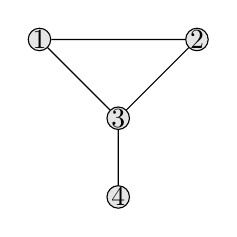
\begin{tikzpicture}[vertex/.style={circle, draw, fill=gray!20, minimum size=2mm, inner sep=0pt}]
        \node[vertex] (v1)  at (-1,2) {$1$};
        \node[vertex] (v2)  at (1,2)  {$2$};
        \node[vertex] (v3)  at (0,1)  {$3$};
        \node[vertex] (v4)  at (0,0)  {$4$};

        \draw (v4)--(v3)--(v1)--(v2)--(v3);
        \end{tikzpicture}
        \end{center}
        $A=
        \begin{pmatrix}
        0 & 1 & 0 & 1 \\
        1 & 0 & 1 & 1 \\
        0 & 1 & 0 & 0 \\
        1 & 1 & 0 & 0
        \end{pmatrix}$
        \begin{itemize}
            \item $v_1$: $v_2, v_4$
            \item $v_2$: $v_1, v_3, v_4$
            \item $v_3$: $v_2$
            \item $v_4$: $v_1, v_2$
        \end{itemize}
\end{example}
\vspace{0.5cm}

\begin{remark}\label{1.20}
\hfill \\
    Memory requirement: \par
    Adjacency matrix: $\theta (n^2)$\par
    Adjacency list: $\theta (n+m)$, where $m$ is the number of edges
\end{remark}